\documentclass[1p]{elsarticle_modified}
%\bibliographystyle{elsarticle-num}

%\usepackage[colorlinks]{hyperref}
%\usepackage{abbrmath_seonhwa} %\Abb, \Ascr, \Acal ,\Abf, \Afrak
\usepackage{amsfonts}
\usepackage{amssymb}
\usepackage{amsmath}
\usepackage{amsthm}
\usepackage{scalefnt}
\usepackage{amsbsy}
\usepackage{kotex}
\usepackage{caption}
\usepackage{subfig}
\usepackage{color}
\usepackage{graphicx}
\usepackage{xcolor} %% white, black, red, green, blue, cyan, magenta, yellow
\usepackage{float}
\usepackage{setspace}
\usepackage{hyperref}

\usepackage{tikz}
\usetikzlibrary{arrows}

\usepackage{multirow}
\usepackage{array} % fixed length table
\usepackage{hhline}

%%%%%%%%%%%%%%%%%%%%%
\makeatletter
\renewcommand*\env@matrix[1][\arraystretch]{%
	\edef\arraystretch{#1}%
	\hskip -\arraycolsep
	\let\@ifnextchar\new@ifnextchar
	\array{*\c@MaxMatrixCols c}}
\makeatother %https://tex.stackexchange.com/questions/14071/how-can-i-increase-the-line-spacing-in-a-matrix
%%%%%%%%%%%%%%%

\usepackage[normalem]{ulem}

\newcommand{\msout}[1]{\ifmmode\text{\sout{\ensuremath{#1}}}\else\sout{#1}\fi}
%SOURCE: \msout is \stkout macro in https://tex.stackexchange.com/questions/20609/strikeout-in-math-mode

\newcommand{\cancel}[1]{
	\ifmmode
	{\color{red}\msout{#1}}
	\else
	{\color{red}\sout{#1}}
	\fi
}

\newcommand{\add}[1]{
	{\color{blue}\uwave{#1}}
}

\newcommand{\replace}[2]{
	\ifmmode
	{\color{red}\msout{#1}}{\color{blue}\uwave{#2}}
	\else
	{\color{red}\sout{#1}}{\color{blue}\uwave{#2}}
	\fi
}

\newcommand{\Sol}{\mathcal{S}} %segment
\newcommand{\D}{D} %diagram
\newcommand{\A}{\mathcal{A}} %arc


%%%%%%%%%%%%%%%%%%%%%%%%%%%%%5 test

\def\sl{\operatorname{\textup{SL}}(2,\Cbb)}
\def\psl{\operatorname{\textup{PSL}}(2,\Cbb)}
\def\quan{\mkern 1mu \triangleright \mkern 1mu}

\theoremstyle{definition}
\newtheorem{thm}{Theorem}[section]
\newtheorem{prop}[thm]{Proposition}
\newtheorem{lem}[thm]{Lemma}
\newtheorem{ques}[thm]{Question}
\newtheorem{cor}[thm]{Corollary}
\newtheorem{defn}[thm]{Definition}
\newtheorem{exam}[thm]{Example}
\newtheorem{rmk}[thm]{Remark}
\newtheorem{alg}[thm]{Algorithm}

\newcommand{\I}{\sqrt{-1}}
\begin{document}

%\begin{frontmatter}
%
%\title{Boundary parabolic representations of knots up to 8 crossings}
%
%%% Group authors per affiliation:
%\author{Yunhi Cho} 
%\address{Department of Mathematics, University of Seoul, Seoul, Korea}
%\ead{yhcho@uos.ac.kr}
%
%
%\author{Seonhwa Kim} %\fnref{s_kim}}
%\address{Center for Geometry and Physics, Institute for Basic Science, Pohang, 37673, Korea}
%\ead{ryeona17@ibs.re.kr}
%
%\author{Hyuk Kim}
%\address{Department of Mathematical Sciences, Seoul National University, Seoul 08826, Korea}
%\ead{hyukkim@snu.ac.kr}
%
%\author{Seokbeom Yoon}
%\address{Department of Mathematical Sciences, Seoul National University, Seoul, 08826,  Korea}
%\ead{sbyoon15@snu.ac.kr}
%
%\begin{abstract}
%We find all boundary parabolic representation of knots up to 8 crossings.
%
%\end{abstract}
%\begin{keyword}
%    \MSC[2010] 57M25 
%\end{keyword}
%
%\end{frontmatter}

%\linenumbers
%\tableofcontents
%
\newcommand\colored[1]{\textcolor{white}{\rule[-0.35ex]{0.8em}{1.4ex}}\kern-0.8em\color{red} #1}%
%\newcommand\colored[1]{\textcolor{white}{ #1}\kern-2.17ex	\textcolor{white}{ #1}\kern-1.81ex	\textcolor{white}{ #1}\kern-2.15ex\color{red}#1	}

{\Large $\underline{12a_{0954}~(K12a_{0954})}$}

\setlength{\tabcolsep}{10pt}
\renewcommand{\arraystretch}{1.6}
\vspace{1cm}\begin{tabular}{m{100pt}>{\centering\arraybackslash}m{274pt}}
\multirow{5}{120pt}{
	\centering
	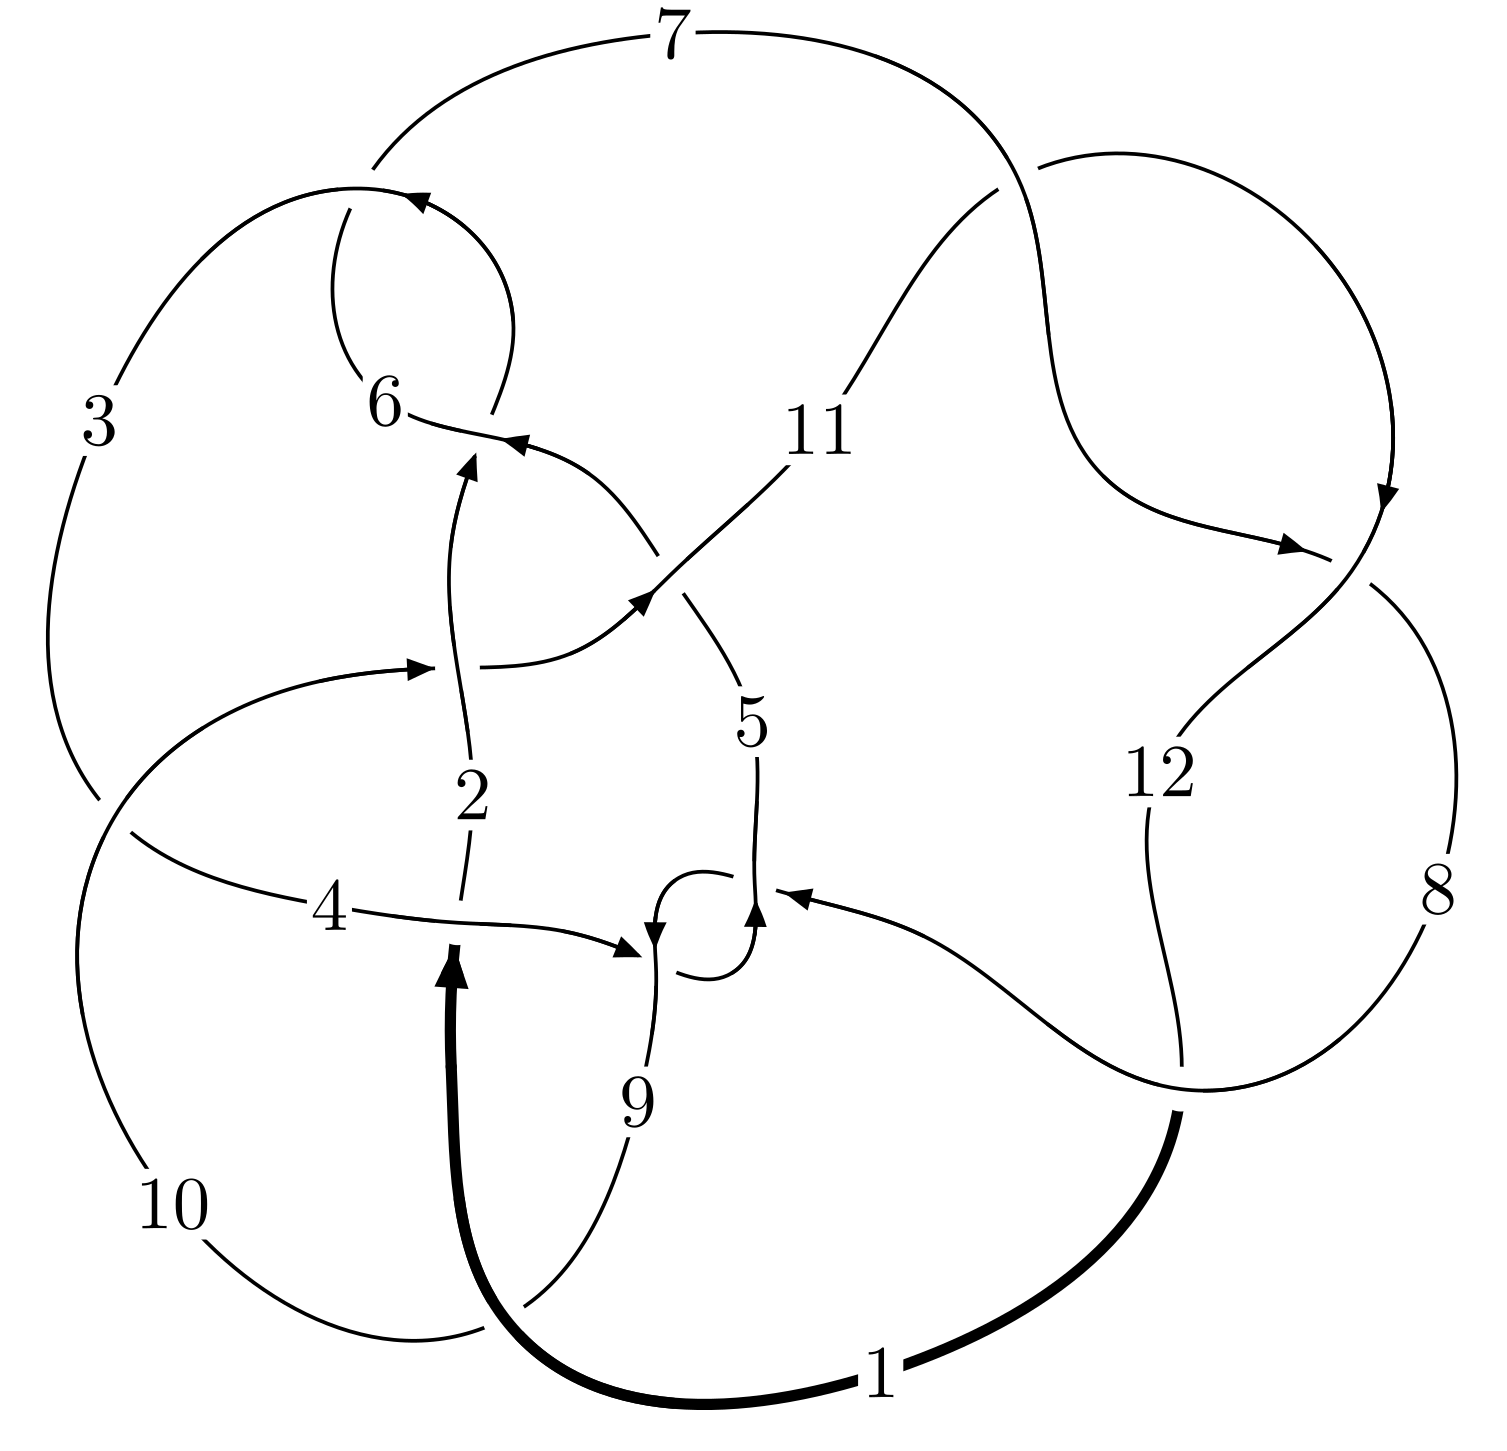
\includegraphics[width=112pt]{../../../GIT/diagram.site/Diagrams/png/1755_12a_0954.png}\\
\ \ \ A knot diagram\footnotemark}&
\allowdisplaybreaks
\textbf{Linearized knot diagam} \\
\cline{2-2}
 &
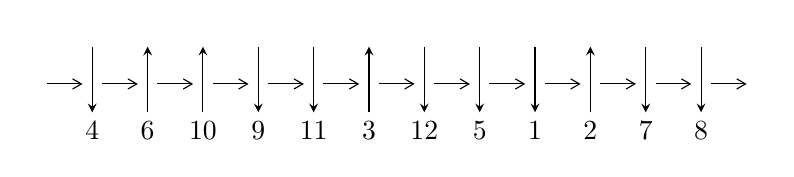
\begin{tikzpicture}[x=20pt, y=17pt]
	% nodes
	\node (C0) at (0, 0) {};
	\node (C1) at (1, 0) {};
	\node (C1U) at (1, +1) {};
	\node (C1D) at (1, -1) {4};

	\node (C2) at (2, 0) {};
	\node (C2U) at (2, +1) {};
	\node (C2D) at (2, -1) {6};

	\node (C3) at (3, 0) {};
	\node (C3U) at (3, +1) {};
	\node (C3D) at (3, -1) {10};

	\node (C4) at (4, 0) {};
	\node (C4U) at (4, +1) {};
	\node (C4D) at (4, -1) {9};

	\node (C5) at (5, 0) {};
	\node (C5U) at (5, +1) {};
	\node (C5D) at (5, -1) {11};

	\node (C6) at (6, 0) {};
	\node (C6U) at (6, +1) {};
	\node (C6D) at (6, -1) {3};

	\node (C7) at (7, 0) {};
	\node (C7U) at (7, +1) {};
	\node (C7D) at (7, -1) {12};

	\node (C8) at (8, 0) {};
	\node (C8U) at (8, +1) {};
	\node (C8D) at (8, -1) {5};

	\node (C9) at (9, 0) {};
	\node (C9U) at (9, +1) {};
	\node (C9D) at (9, -1) {1};

	\node (C10) at (10, 0) {};
	\node (C10U) at (10, +1) {};
	\node (C10D) at (10, -1) {2};

	\node (C11) at (11, 0) {};
	\node (C11U) at (11, +1) {};
	\node (C11D) at (11, -1) {7};

	\node (C12) at (12, 0) {};
	\node (C12U) at (12, +1) {};
	\node (C12D) at (12, -1) {8};
	\node (C13) at (13, 0) {};

	% arrows
	\draw[->,>={angle 60}]
	(C0) edge (C1) (C1) edge (C2) (C2) edge (C3) (C3) edge (C4) (C4) edge (C5) (C5) edge (C6) (C6) edge (C7) (C7) edge (C8) (C8) edge (C9) (C9) edge (C10) (C10) edge (C11) (C11) edge (C12) (C12) edge (C13) ;	\draw[->,>=stealth]
	(C1U) edge (C1D) (C2D) edge (C2U) (C3D) edge (C3U) (C4U) edge (C4D) (C5U) edge (C5D) (C6D) edge (C6U) (C7U) edge (C7D) (C8U) edge (C8D) (C9U) edge (C9D) (C10D) edge (C10U) (C11U) edge (C11D) (C12U) edge (C12D) ;
	\end{tikzpicture} \\
\hhline{~~} \\& 
\textbf{Solving Sequence} \\ \cline{2-2} 
 &
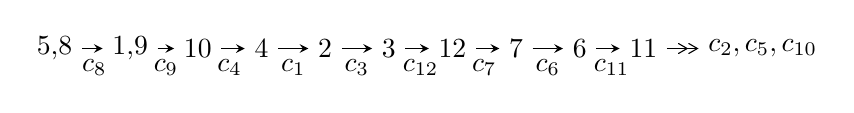
\begin{tikzpicture}[x=23pt, y=7pt]
	% node
	\node (A0) at (-1/8, 0) {5,8};
	\node (A1) at (17/16, 0) {1,9};
	\node (A2) at (17/8, 0) {10};
	\node (A3) at (25/8, 0) {4};
	\node (A4) at (33/8, 0) {2};
	\node (A5) at (41/8, 0) {3};
	\node (A6) at (49/8, 0) {12};
	\node (A7) at (57/8, 0) {7};
	\node (A8) at (65/8, 0) {6};
	\node (A9) at (73/8, 0) {11};
	\node (C1) at (1/2, -1) {$c_{8}$};
	\node (C2) at (13/8, -1) {$c_{9}$};
	\node (C3) at (21/8, -1) {$c_{4}$};
	\node (C4) at (29/8, -1) {$c_{1}$};
	\node (C5) at (37/8, -1) {$c_{3}$};
	\node (C6) at (45/8, -1) {$c_{12}$};
	\node (C7) at (53/8, -1) {$c_{7}$};
	\node (C8) at (61/8, -1) {$c_{6}$};
	\node (C9) at (69/8, -1) {$c_{11}$};
	\node (A10) at (11, 0) {$c_{2},c_{5},c_{10}$};

	% edge
	\draw[->,>=stealth]	
	(A0) edge (A1) (A1) edge (A2) (A2) edge (A3) (A3) edge (A4) (A4) edge (A5) (A5) edge (A6) (A6) edge (A7) (A7) edge (A8) (A8) edge (A9) ;
	\draw[->>,>={angle 60}]	
	(A9) edge (A10);
\end{tikzpicture} \\ 

\end{tabular} \\

\footnotetext{
The image of knot diagram is generated by the software ``\textbf{Draw programme}" developed by Andrew Bartholomew(\url{http://www.layer8.co.uk/maths/draw/index.htm\#Running-draw}), where we modified some parts for our purpose(\url{https://github.com/CATsTAILs/LinksPainter}).
}\phantom \\ \newline 
\centering \textbf{Ideals for irreducible components\footnotemark of $X_{\text{par}}$} 
 
\begin{align*}
I^u_{1}&=\langle 
7.34935\times10^{686} u^{138}+3.18871\times10^{687} u^{137}+\cdots+2.74628\times10^{687} b+7.47276\times10^{689},\\
\phantom{I^u_{1}}&\phantom{= \langle  }3.96893\times10^{689} u^{138}+1.01996\times10^{690} u^{137}+\cdots+4.23751\times10^{690} a-1.16664\times10^{693},\\
\phantom{I^u_{1}}&\phantom{= \langle  }u^{139}+4 u^{138}+\cdots+10765 u+1543\rangle \\
I^u_{2}&=\langle 
2.42322\times10^{20} u^{33}-2.34759\times10^{21} u^{32}+\cdots+1.44163\times10^{21} b-2.34593\times10^{21},\\
\phantom{I^u_{2}}&\phantom{= \langle  }7.15733\times10^{18} u^{33}+2.04516\times10^{19} u^{32}+\cdots+7.87774\times10^{18} a-1.30471\times10^{19},\;u^{34}- u^{33}+\cdots-2 u+1\rangle \\
\\
\end{align*}
\raggedright * 2 irreducible components of $\dim_{\mathbb{C}}=0$, with total 173 representations.\\
\footnotetext{All coefficients of polynomials are rational numbers. But the coefficients are sometimes approximated in decimal forms when there is not enough margin.}
\newpage
\renewcommand{\arraystretch}{1}
\centering \section*{I. $I^u_{1}= \langle 7.35\times10^{686} u^{138}+3.19\times10^{687} u^{137}+\cdots+2.75\times10^{687} b+7.47\times10^{689},\;3.97\times10^{689} u^{138}+1.02\times10^{690} u^{137}+\cdots+4.24\times10^{690} a-1.17\times10^{693},\;u^{139}+4 u^{138}+\cdots+10765 u+1543 \rangle$}
\flushleft \textbf{(i) Arc colorings}\\
\begin{tabular}{m{7pt} m{180pt} m{7pt} m{180pt} }
\flushright $a_{5}=$&$\begin{pmatrix}0\\u\end{pmatrix}$ \\
\flushright $a_{8}=$&$\begin{pmatrix}1\\0\end{pmatrix}$ \\
\flushright $a_{1}=$&$\begin{pmatrix}-0.0936618 u^{138}-0.240697 u^{137}+\cdots+1753.34 u+275.314\\-0.267611 u^{138}-1.16110 u^{137}+\cdots-2455.08 u-272.105\end{pmatrix}$ \\
\flushright $a_{9}=$&$\begin{pmatrix}1\\u^2\end{pmatrix}$ \\
\flushright $a_{10}=$&$\begin{pmatrix}0.172908 u^{138}+0.100924 u^{137}+\cdots-9074.58 u-1380.96\\0.524853 u^{138}+2.04517 u^{137}+\cdots+1010.16 u-20.9051\end{pmatrix}$ \\
\flushright $a_{4}=$&$\begin{pmatrix}u\\u^3+u\end{pmatrix}$ \\
\flushright $a_{2}=$&$\begin{pmatrix}-0.264885 u^{138}-0.991986 u^{137}+\cdots+16.6171 u+80.4220\\-0.320116 u^{138}-1.40709 u^{137}+\cdots-3212.85 u-364.547\end{pmatrix}$ \\
\flushright $a_{3}=$&$\begin{pmatrix}-0.412145 u^{138}-1.56850 u^{137}+\cdots-45.6170 u+182.029\\-0.473335 u^{138}-2.41050 u^{137}+\cdots-9853.94 u-1272.53\end{pmatrix}$ \\
\flushright $a_{12}=$&$\begin{pmatrix}-0.361273 u^{138}-1.40180 u^{137}+\cdots-701.737 u+3.20887\\-0.267611 u^{138}-1.16110 u^{137}+\cdots-2455.08 u-272.105\end{pmatrix}$ \\
\flushright $a_{7}=$&$\begin{pmatrix}-0.510251 u^{138}-1.80085 u^{137}+\cdots+1914.90 u+431.443\\-0.591229 u^{138}-2.68575 u^{137}+\cdots-7174.16 u-844.702\end{pmatrix}$ \\
\flushright $a_{6}=$&$\begin{pmatrix}0.302426 u^{138}+1.57715 u^{137}+\cdots+6649.40 u+813.536\\0.891376 u^{138}+3.49644 u^{137}+\cdots+495.277 u-220.580\end{pmatrix}$ \\
\flushright $a_{11}=$&$\begin{pmatrix}0.300992 u^{138}+0.692750 u^{137}+\cdots-6844.57 u-1086.16\\0.998380 u^{138}+4.67724 u^{137}+\cdots+14271.2 u+1727.14\end{pmatrix}$\\&\end{tabular}
\flushleft \textbf{(ii) Obstruction class $= -1$}\\~\\
\flushleft \textbf{(iii) Cusp Shapes $= 2.33258 u^{138}+5.97100 u^{137}+\cdots-47823.9 u-7695.64$}\\~\\
\newpage\renewcommand{\arraystretch}{1}
\flushleft \textbf{(iv) u-Polynomials at the component}\newline \\
\begin{tabular}{m{50pt}|m{274pt}}
Crossings & \hspace{64pt}u-Polynomials at each crossing \\
\hline $$\begin{aligned}c_{1}\end{aligned}$$&$\begin{aligned}
&u^{139}-10 u^{138}+\cdots+668505 u-38071
\end{aligned}$\\
\hline $$\begin{aligned}c_{2},c_{6}\end{aligned}$$&$\begin{aligned}
&u^{139}-6 u^{138}+\cdots+73 u+1721
\end{aligned}$\\
\hline $$\begin{aligned}c_{3}\end{aligned}$$&$\begin{aligned}
&u^{139}+u^{138}+\cdots+3238 u+389
\end{aligned}$\\
\hline $$\begin{aligned}c_{4},c_{8}\end{aligned}$$&$\begin{aligned}
&u^{139}+4 u^{138}+\cdots+10765 u+1543
\end{aligned}$\\
\hline $$\begin{aligned}c_{5}\end{aligned}$$&$\begin{aligned}
&u^{139}+u^{138}+\cdots-112549 u+43381
\end{aligned}$\\
\hline $$\begin{aligned}c_{7},c_{11},c_{12}\end{aligned}$$&$\begin{aligned}
&u^{139}- u^{138}+\cdots-629 u+71
\end{aligned}$\\
\hline $$\begin{aligned}c_{9}\end{aligned}$$&$\begin{aligned}
&u^{139}+3 u^{138}+\cdots-19 u+1
\end{aligned}$\\
\hline $$\begin{aligned}c_{10}\end{aligned}$$&$\begin{aligned}
&u^{139}+7 u^{138}+\cdots+685122 u+90743
\end{aligned}$\\
\hline
\end{tabular}\\~\\
\newpage\renewcommand{\arraystretch}{1}
\flushleft \textbf{(v) Riley Polynomials at the component}\newline \\
\begin{tabular}{m{50pt}|m{274pt}}
Crossings & \hspace{64pt}Riley Polynomials at each crossing \\
\hline $$\begin{aligned}c_{1}\end{aligned}$$&$\begin{aligned}
&y^{139}+46 y^{138}+\cdots-59985059471 y-1449401041
\end{aligned}$\\
\hline $$\begin{aligned}c_{2},c_{6}\end{aligned}$$&$\begin{aligned}
&y^{139}-74 y^{138}+\cdots+121225685 y-2961841
\end{aligned}$\\
\hline $$\begin{aligned}c_{3}\end{aligned}$$&$\begin{aligned}
&y^{139}+27 y^{138}+\cdots-3405768 y-151321
\end{aligned}$\\
\hline $$\begin{aligned}c_{4},c_{8}\end{aligned}$$&$\begin{aligned}
&y^{139}+94 y^{138}+\cdots-45669961 y-2380849
\end{aligned}$\\
\hline $$\begin{aligned}c_{5}\end{aligned}$$&$\begin{aligned}
&y^{139}+15 y^{138}+\cdots-293305335987 y-1881911161
\end{aligned}$\\
\hline $$\begin{aligned}c_{7},c_{11},c_{12}\end{aligned}$$&$\begin{aligned}
&y^{139}-145 y^{138}+\cdots+23317 y-5041
\end{aligned}$\\
\hline $$\begin{aligned}c_{9}\end{aligned}$$&$\begin{aligned}
&y^{139}-11 y^{138}+\cdots+31 y-1
\end{aligned}$\\
\hline $$\begin{aligned}c_{10}\end{aligned}$$&$\begin{aligned}
&y^{139}-51 y^{138}+\cdots+9380316628 y-8234292049
\end{aligned}$\\
\hline
\end{tabular}\\~\\
\newpage\flushleft \textbf{(vi) Complex Volumes and Cusp Shapes}
$$\begin{array}{c|c|c}  
\text{Solutions to }I^u_{1}& \I (\text{vol} + \sqrt{-1}CS) & \text{Cusp shape}\\
 \hline 
\begin{aligned}
u &= -0.984345 + 0.163711 I \\
a &= \phantom{-}0.317362 - 0.123113 I \\
b &= -0.405404 + 0.328192 I\end{aligned}
 & -1.61926 + 3.70744 I & \phantom{-0.000000 } 0 \\ \hline\begin{aligned}
u &= -0.984345 - 0.163711 I \\
a &= \phantom{-}0.317362 + 0.123113 I \\
b &= -0.405404 - 0.328192 I\end{aligned}
 & -1.61926 - 3.70744 I & \phantom{-0.000000 } 0 \\ \hline\begin{aligned}
u &= -0.858886 + 0.521143 I \\
a &= -0.034798 + 0.336032 I \\
b &= \phantom{-}1.50776 + 0.23002 I\end{aligned}
 & -5.00542 - 5.88034 I & \phantom{-0.000000 } 0 \\ \hline\begin{aligned}
u &= -0.858886 - 0.521143 I \\
a &= -0.034798 - 0.336032 I \\
b &= \phantom{-}1.50776 - 0.23002 I\end{aligned}
 & -5.00542 + 5.88034 I & \phantom{-0.000000 } 0 \\ \hline\begin{aligned}
u &= \phantom{-}0.967502 + 0.072523 I \\
a &= -0.494935 - 0.148784 I \\
b &= -1.56393 + 0.08436 I\end{aligned}
 & -8.84824 + 0.83629 I & \phantom{-0.000000 } 0 \\ \hline\begin{aligned}
u &= \phantom{-}0.967502 - 0.072523 I \\
a &= -0.494935 + 0.148784 I \\
b &= -1.56393 - 0.08436 I\end{aligned}
 & -8.84824 - 0.83629 I & \phantom{-0.000000 } 0 \\ \hline\begin{aligned}
u &= -0.173315 + 1.019320 I \\
a &= \phantom{-}0.25912 + 2.25416 I \\
b &= \phantom{-}1.46511 - 0.24456 I\end{aligned}
 & \phantom{-}0.57027 + 8.62979 I & \phantom{-0.000000 } 0 \\ \hline\begin{aligned}
u &= -0.173315 - 1.019320 I \\
a &= \phantom{-}0.25912 - 2.25416 I \\
b &= \phantom{-}1.46511 + 0.24456 I\end{aligned}
 & \phantom{-}0.57027 - 8.62979 I & \phantom{-0.000000 } 0 \\ \hline\begin{aligned}
u &= \phantom{-}0.209486 + 1.012630 I \\
a &= \phantom{-}0.01204 - 1.73362 I \\
b &= \phantom{-}1.45610 + 0.18075 I\end{aligned}
 & -2.24906 - 3.84323 I & \phantom{-0.000000 } 0 \\ \hline\begin{aligned}
u &= \phantom{-}0.209486 - 1.012630 I \\
a &= \phantom{-}0.01204 + 1.73362 I \\
b &= \phantom{-}1.45610 - 0.18075 I\end{aligned}
 & -2.24906 + 3.84323 I & \phantom{-0.000000 } 0\\
 \hline 
 \end{array}$$\newpage$$\begin{array}{c|c|c}  
\text{Solutions to }I^u_{1}& \I (\text{vol} + \sqrt{-1}CS) & \text{Cusp shape}\\
 \hline 
\begin{aligned}
u &= -0.867416 + 0.421365 I \\
a &= \phantom{-}0.607270 - 0.176153 I \\
b &= \phantom{-}0.786540 + 0.184391 I\end{aligned}
 & \phantom{-}1.30510 - 1.99753 I & \phantom{-0.000000 } 0 \\ \hline\begin{aligned}
u &= -0.867416 - 0.421365 I \\
a &= \phantom{-}0.607270 + 0.176153 I \\
b &= \phantom{-}0.786540 - 0.184391 I\end{aligned}
 & \phantom{-}1.30510 + 1.99753 I & \phantom{-0.000000 } 0 \\ \hline\begin{aligned}
u &= -0.177876 + 0.947063 I \\
a &= \phantom{-}0.701272 + 1.190700 I \\
b &= \phantom{-}1.328990 - 0.174052 I\end{aligned}
 & \phantom{-}1.83948 + 0.31019 I & \phantom{-0.000000 } 0 \\ \hline\begin{aligned}
u &= -0.177876 - 0.947063 I \\
a &= \phantom{-}0.701272 - 1.190700 I \\
b &= \phantom{-}1.328990 + 0.174052 I\end{aligned}
 & \phantom{-}1.83948 - 0.31019 I & \phantom{-0.000000 } 0 \\ \hline\begin{aligned}
u &= \phantom{-}0.948364 + 0.114684 I \\
a &= \phantom{-}0.254988 + 0.113237 I \\
b &= -0.525303 - 0.601669 I\end{aligned}
 & \phantom{-}1.80221 - 9.27217 I & \phantom{-0.000000 } 0 \\ \hline\begin{aligned}
u &= \phantom{-}0.948364 - 0.114684 I \\
a &= \phantom{-}0.254988 - 0.113237 I \\
b &= -0.525303 + 0.601669 I\end{aligned}
 & \phantom{-}1.80221 + 9.27217 I & \phantom{-0.000000 } 0 \\ \hline\begin{aligned}
u &= \phantom{-}0.947563 + 0.054813 I \\
a &= \phantom{-}0.329502 + 0.114601 I \\
b &= \phantom{-}0.065641 - 0.525613 I\end{aligned}
 & \phantom{-}3.76074 + 0.63220 I & \phantom{-0.000000 } 0 \\ \hline\begin{aligned}
u &= \phantom{-}0.947563 - 0.054813 I \\
a &= \phantom{-}0.329502 - 0.114601 I \\
b &= \phantom{-}0.065641 + 0.525613 I\end{aligned}
 & \phantom{-}3.76074 - 0.63220 I & \phantom{-0.000000 } 0 \\ \hline\begin{aligned}
u &= -0.345652 + 1.007400 I \\
a &= -0.87690 + 1.35211 I \\
b &= \phantom{-}1.46787 - 0.59646 I\end{aligned}
 & -3.10394 + 3.05580 I & \phantom{-0.000000 } 0 \\ \hline\begin{aligned}
u &= -0.345652 - 1.007400 I \\
a &= -0.87690 - 1.35211 I \\
b &= \phantom{-}1.46787 + 0.59646 I\end{aligned}
 & -3.10394 - 3.05580 I & \phantom{-0.000000 } 0\\
 \hline 
 \end{array}$$\newpage$$\begin{array}{c|c|c}  
\text{Solutions to }I^u_{1}& \I (\text{vol} + \sqrt{-1}CS) & \text{Cusp shape}\\
 \hline 
\begin{aligned}
u &= -0.665495 + 0.832437 I \\
a &= \phantom{-}0.597877 + 0.524581 I \\
b &= -0.289783 - 0.387641 I\end{aligned}
 & -0.92855 + 2.86098 I & \phantom{-0.000000 } 0 \\ \hline\begin{aligned}
u &= -0.665495 - 0.832437 I \\
a &= \phantom{-}0.597877 - 0.524581 I \\
b &= -0.289783 + 0.387641 I\end{aligned}
 & -0.92855 - 2.86098 I & \phantom{-0.000000 } 0 \\ \hline\begin{aligned}
u &= -0.416651 + 1.004640 I \\
a &= -0.17056 - 1.70837 I \\
b &= -0.400838 + 0.074764 I\end{aligned}
 & \phantom{-}2.92086 + 6.73817 I & \phantom{-0.000000 } 0 \\ \hline\begin{aligned}
u &= -0.416651 - 1.004640 I \\
a &= -0.17056 + 1.70837 I \\
b &= -0.400838 - 0.074764 I\end{aligned}
 & \phantom{-}2.92086 - 6.73817 I & \phantom{-0.000000 } 0 \\ \hline\begin{aligned}
u &= \phantom{-}0.328815 + 1.040940 I \\
a &= -1.03808 - 1.10020 I \\
b &= \phantom{-}1.72147 + 0.32756 I\end{aligned}
 & -3.06181 - 0.42276 I & \phantom{-0.000000 } 0 \\ \hline\begin{aligned}
u &= \phantom{-}0.328815 - 1.040940 I \\
a &= -1.03808 + 1.10020 I \\
b &= \phantom{-}1.72147 - 0.32756 I\end{aligned}
 & -3.06181 + 0.42276 I & \phantom{-0.000000 } 0 \\ \hline\begin{aligned}
u &= \phantom{-}0.298772 + 1.050800 I \\
a &= \phantom{-}0.13707 + 1.55026 I \\
b &= \phantom{-}0.124904 - 0.263502 I\end{aligned}
 & \phantom{-}1.30186 - 3.91353 I & \phantom{-0.000000 } 0 \\ \hline\begin{aligned}
u &= \phantom{-}0.298772 - 1.050800 I \\
a &= \phantom{-}0.13707 - 1.55026 I \\
b &= \phantom{-}0.124904 + 0.263502 I\end{aligned}
 & \phantom{-}1.30186 + 3.91353 I & \phantom{-0.000000 } 0 \\ \hline\begin{aligned}
u &= -0.903951 + 0.035507 I \\
a &= -0.334684 + 0.266905 I \\
b &= -1.49079 - 0.18892 I\end{aligned}
 & -7.63137 - 5.02257 I & \phantom{-0.000000 } 0 \\ \hline\begin{aligned}
u &= -0.903951 - 0.035507 I \\
a &= -0.334684 - 0.266905 I \\
b &= -1.49079 + 0.18892 I\end{aligned}
 & -7.63137 + 5.02257 I & \phantom{-0.000000 } 0\\
 \hline 
 \end{array}$$\newpage$$\begin{array}{c|c|c}  
\text{Solutions to }I^u_{1}& \I (\text{vol} + \sqrt{-1}CS) & \text{Cusp shape}\\
 \hline 
\begin{aligned}
u &= \phantom{-}0.305158 + 0.816887 I \\
a &= \phantom{-}0.33859 - 1.71210 I \\
b &= \phantom{-}0.241817 + 1.118750 I\end{aligned}
 & \phantom{-}2.35998 - 5.79520 I & \phantom{-0.000000 } 0 \\ \hline\begin{aligned}
u &= \phantom{-}0.305158 - 0.816887 I \\
a &= \phantom{-}0.33859 + 1.71210 I \\
b &= \phantom{-}0.241817 - 1.118750 I\end{aligned}
 & \phantom{-}2.35998 + 5.79520 I & \phantom{-0.000000 } 0 \\ \hline\begin{aligned}
u &= \phantom{-}0.820846 + 0.267285 I \\
a &= -1.075110 - 0.400041 I \\
b &= -1.59964 + 0.01315 I\end{aligned}
 & -6.77889 + 2.54045 I & \phantom{-0.000000 } 0 \\ \hline\begin{aligned}
u &= \phantom{-}0.820846 - 0.267285 I \\
a &= -1.075110 + 0.400041 I \\
b &= -1.59964 - 0.01315 I\end{aligned}
 & -6.77889 - 2.54045 I & \phantom{-0.000000 } 0 \\ \hline\begin{aligned}
u &= \phantom{-}0.846059 + 0.764034 I \\
a &= -0.064795 - 0.277890 I \\
b &= \phantom{-}1.45640 - 0.15711 I\end{aligned}
 & -6.79054 - 0.70134 I & \phantom{-0.000000 } 0 \\ \hline\begin{aligned}
u &= \phantom{-}0.846059 - 0.764034 I \\
a &= -0.064795 + 0.277890 I \\
b &= \phantom{-}1.45640 + 0.15711 I\end{aligned}
 & -6.79054 + 0.70134 I & \phantom{-0.000000 } 0 \\ \hline\begin{aligned}
u &= -0.410065 + 0.753558 I \\
a &= \phantom{-}0.257721 + 1.114800 I \\
b &= \phantom{-}0.280895 - 0.583056 I\end{aligned}
 & -0.90606 + 1.55341 I & \phantom{-0.000000 } 0 \\ \hline\begin{aligned}
u &= -0.410065 - 0.753558 I \\
a &= \phantom{-}0.257721 - 1.114800 I \\
b &= \phantom{-}0.280895 + 0.583056 I\end{aligned}
 & -0.90606 - 1.55341 I & \phantom{-0.000000 } 0 \\ \hline\begin{aligned}
u &= \phantom{-}0.663817 + 0.931200 I \\
a &= \phantom{-}0.02898 + 1.54162 I \\
b &= -1.41554 - 0.29313 I\end{aligned}
 & -6.21862 - 4.94337 I & \phantom{-0.000000 } 0 \\ \hline\begin{aligned}
u &= \phantom{-}0.663817 - 0.931200 I \\
a &= \phantom{-}0.02898 - 1.54162 I \\
b &= -1.41554 + 0.29313 I\end{aligned}
 & -6.21862 + 4.94337 I & \phantom{-0.000000 } 0\\
 \hline 
 \end{array}$$\newpage$$\begin{array}{c|c|c}  
\text{Solutions to }I^u_{1}& \I (\text{vol} + \sqrt{-1}CS) & \text{Cusp shape}\\
 \hline 
\begin{aligned}
u &= -0.055156 + 0.848071 I \\
a &= \phantom{-}0.81299 - 1.50904 I \\
b &= -0.485747 + 0.310112 I\end{aligned}
 & \phantom{-}1.85993 + 1.66350 I & \phantom{-0.000000 } 0 \\ \hline\begin{aligned}
u &= -0.055156 - 0.848071 I \\
a &= \phantom{-}0.81299 + 1.50904 I \\
b &= -0.485747 - 0.310112 I\end{aligned}
 & \phantom{-}1.85993 - 1.66350 I & \phantom{-0.000000 } 0 \\ \hline\begin{aligned}
u &= -0.120590 + 0.837860 I \\
a &= \phantom{-}0.53710 - 2.73606 I \\
b &= -1.311550 - 0.073495 I\end{aligned}
 & -0.15517 - 7.25854 I & \phantom{-0.000000 } 0 \\ \hline\begin{aligned}
u &= -0.120590 - 0.837860 I \\
a &= \phantom{-}0.53710 + 2.73606 I \\
b &= -1.311550 + 0.073495 I\end{aligned}
 & -0.15517 + 7.25854 I & \phantom{-0.000000 } 0 \\ \hline\begin{aligned}
u &= -0.239360 + 0.811073 I \\
a &= \phantom{-}0.67104 - 2.24339 I \\
b &= -1.024730 + 0.221853 I\end{aligned}
 & \phantom{-}1.54634 + 1.64211 I & \phantom{-0.000000 } 0 \\ \hline\begin{aligned}
u &= -0.239360 - 0.811073 I \\
a &= \phantom{-}0.67104 + 2.24339 I \\
b &= -1.024730 - 0.221853 I\end{aligned}
 & \phantom{-}1.54634 - 1.64211 I & \phantom{-0.000000 } 0 \\ \hline\begin{aligned}
u &= \phantom{-}0.269501 + 1.126440 I \\
a &= -0.168913 + 1.115810 I \\
b &= \phantom{-}0.666706 - 0.630340 I\end{aligned}
 & \phantom{-}2.03934 - 3.87980 I & \phantom{-0.000000 } 0 \\ \hline\begin{aligned}
u &= \phantom{-}0.269501 - 1.126440 I \\
a &= -0.168913 - 1.115810 I \\
b &= \phantom{-}0.666706 + 0.630340 I\end{aligned}
 & \phantom{-}2.03934 + 3.87980 I & \phantom{-0.000000 } 0 \\ \hline\begin{aligned}
u &= \phantom{-}0.320024 + 1.120450 I \\
a &= -0.09647 + 1.68783 I \\
b &= -0.137077 - 1.008610 I\end{aligned}
 & \phantom{-}1.58535 - 5.28364 I & \phantom{-0.000000 } 0 \\ \hline\begin{aligned}
u &= \phantom{-}0.320024 - 1.120450 I \\
a &= -0.09647 - 1.68783 I \\
b &= -0.137077 + 1.008610 I\end{aligned}
 & \phantom{-}1.58535 + 5.28364 I & \phantom{-0.000000 } 0\\
 \hline 
 \end{array}$$\newpage$$\begin{array}{c|c|c}  
\text{Solutions to }I^u_{1}& \I (\text{vol} + \sqrt{-1}CS) & \text{Cusp shape}\\
 \hline 
\begin{aligned}
u &= \phantom{-}0.317984 + 1.122460 I \\
a &= -0.95229 - 1.24699 I \\
b &= \phantom{-}1.49185 + 0.10434 I\end{aligned}
 & -4.52917 - 3.20075 I & \phantom{-0.000000 } 0 \\ \hline\begin{aligned}
u &= \phantom{-}0.317984 - 1.122460 I \\
a &= -0.95229 + 1.24699 I \\
b &= \phantom{-}1.49185 - 0.10434 I\end{aligned}
 & -4.52917 + 3.20075 I & \phantom{-0.000000 } 0 \\ \hline\begin{aligned}
u &= -0.306639 + 1.126310 I \\
a &= \phantom{-}0.20136 - 1.64185 I \\
b &= -0.565466 + 0.757861 I\end{aligned}
 & \phantom{-}1.98266 + 2.53406 I & \phantom{-0.000000 } 0 \\ \hline\begin{aligned}
u &= -0.306639 - 1.126310 I \\
a &= \phantom{-}0.20136 + 1.64185 I \\
b &= -0.565466 - 0.757861 I\end{aligned}
 & \phantom{-}1.98266 - 2.53406 I & \phantom{-0.000000 } 0 \\ \hline\begin{aligned}
u &= \phantom{-}0.013356 + 0.827803 I \\
a &= -0.349403 + 0.562074 I \\
b &= -1.67021 - 0.02537 I\end{aligned}
 & -6.39087 + 2.02065 I & \phantom{-0.000000 } 0 \\ \hline\begin{aligned}
u &= \phantom{-}0.013356 - 0.827803 I \\
a &= -0.349403 - 0.562074 I \\
b &= -1.67021 + 0.02537 I\end{aligned}
 & -6.39087 - 2.02065 I & \phantom{-0.000000 } 0 \\ \hline\begin{aligned}
u &= -0.292769 + 1.138220 I \\
a &= -0.56388 - 1.30126 I \\
b &= \phantom{-}0.764263 + 1.097700 I\end{aligned}
 & \phantom{-}5.68267 + 7.59871 I & \phantom{-0.000000 } 0 \\ \hline\begin{aligned}
u &= -0.292769 - 1.138220 I \\
a &= -0.56388 + 1.30126 I \\
b &= \phantom{-}0.764263 - 1.097700 I\end{aligned}
 & \phantom{-}5.68267 - 7.59871 I & \phantom{-0.000000 } 0 \\ \hline\begin{aligned}
u &= \phantom{-}0.044985 + 1.184420 I \\
a &= -0.160859 - 1.263000 I \\
b &= -0.399145 + 0.580971 I\end{aligned}
 & \phantom{-}3.74587 + 1.13480 I & \phantom{-0.000000 } 0 \\ \hline\begin{aligned}
u &= \phantom{-}0.044985 - 1.184420 I \\
a &= -0.160859 + 1.263000 I \\
b &= -0.399145 - 0.580971 I\end{aligned}
 & \phantom{-}3.74587 - 1.13480 I & \phantom{-0.000000 } 0\\
 \hline 
 \end{array}$$\newpage$$\begin{array}{c|c|c}  
\text{Solutions to }I^u_{1}& \I (\text{vol} + \sqrt{-1}CS) & \text{Cusp shape}\\
 \hline 
\begin{aligned}
u &= -0.591452 + 1.029330 I \\
a &= \phantom{-}0.30372 - 1.57353 I \\
b &= -1.51211 + 0.41168 I\end{aligned}
 & -3.42516 + 11.21010 I & \phantom{-0.000000 } 0 \\ \hline\begin{aligned}
u &= -0.591452 - 1.029330 I \\
a &= \phantom{-}0.30372 + 1.57353 I \\
b &= -1.51211 - 0.41168 I\end{aligned}
 & -3.42516 - 11.21010 I & \phantom{-0.000000 } 0 \\ \hline\begin{aligned}
u &= \phantom{-}0.111053 + 0.799051 I \\
a &= \phantom{-}0.58668 + 2.35867 I \\
b &= -1.322310 - 0.072592 I\end{aligned}
 & -3.16650 + 2.25588 I & \phantom{-0.000000 } 0 \\ \hline\begin{aligned}
u &= \phantom{-}0.111053 - 0.799051 I \\
a &= \phantom{-}0.58668 - 2.35867 I \\
b &= -1.322310 + 0.072592 I\end{aligned}
 & -3.16650 - 2.25588 I & \phantom{-0.000000 } 0 \\ \hline\begin{aligned}
u &= \phantom{-}0.017340 + 1.193460 I \\
a &= -0.63967 + 1.52873 I \\
b &= -0.318717 - 0.660277 I\end{aligned}
 & \phantom{-}6.39748 - 5.33155 I & \phantom{-0.000000 } 0 \\ \hline\begin{aligned}
u &= \phantom{-}0.017340 - 1.193460 I \\
a &= -0.63967 - 1.52873 I \\
b &= -0.318717 + 0.660277 I\end{aligned}
 & \phantom{-}6.39748 + 5.33155 I & \phantom{-0.000000 } 0 \\ \hline\begin{aligned}
u &= -0.002475 + 0.800728 I \\
a &= \phantom{-}1.54046 + 0.42662 I \\
b &= -2.03520 - 0.17589 I\end{aligned}
 & -4.86930 - 1.22848 I & \phantom{-0.000000 } 0 \\ \hline\begin{aligned}
u &= -0.002475 - 0.800728 I \\
a &= \phantom{-}1.54046 - 0.42662 I \\
b &= -2.03520 + 0.17589 I\end{aligned}
 & -4.86930 + 1.22848 I & \phantom{-0.000000 } 0 \\ \hline\begin{aligned}
u &= -0.411807 + 1.127770 I \\
a &= -0.939757 + 1.025840 I \\
b &= \phantom{-}1.339180 - 0.027451 I\end{aligned}
 & -3.92750 - 0.69940 I & \phantom{-0.000000 } 0 \\ \hline\begin{aligned}
u &= -0.411807 - 1.127770 I \\
a &= -0.939757 - 1.025840 I \\
b &= \phantom{-}1.339180 + 0.027451 I\end{aligned}
 & -3.92750 + 0.69940 I & \phantom{-0.000000 } 0\\
 \hline 
 \end{array}$$\newpage$$\begin{array}{c|c|c}  
\text{Solutions to }I^u_{1}& \I (\text{vol} + \sqrt{-1}CS) & \text{Cusp shape}\\
 \hline 
\begin{aligned}
u &= -0.286293 + 1.168760 I \\
a &= -0.464937 - 0.653723 I \\
b &= \phantom{-}1.141310 + 0.599099 I\end{aligned}
 & \phantom{-}4.72297 - 0.88647 I & \phantom{-0.000000 } 0 \\ \hline\begin{aligned}
u &= -0.286293 - 1.168760 I \\
a &= -0.464937 + 0.653723 I \\
b &= \phantom{-}1.141310 - 0.599099 I\end{aligned}
 & \phantom{-}4.72297 + 0.88647 I & \phantom{-0.000000 } 0 \\ \hline\begin{aligned}
u &= -0.764720 + 0.165524 I \\
a &= -0.781745 + 0.770300 I \\
b &= -1.49881 + 0.08202 I\end{aligned}
 & -6.32352 - 0.11113 I & \phantom{-0.000000 } 0 \\ \hline\begin{aligned}
u &= -0.764720 - 0.165524 I \\
a &= -0.781745 - 0.770300 I \\
b &= -1.49881 - 0.08202 I\end{aligned}
 & -6.32352 + 0.11113 I & \phantom{-0.000000 } 0 \\ \hline\begin{aligned}
u &= -0.983411 + 0.788853 I \\
a &= -0.670181 - 0.732094 I \\
b &= -1.343380 - 0.099506 I\end{aligned}
 & -0.51861 - 2.64876 I & \phantom{-0.000000 } 0 \\ \hline\begin{aligned}
u &= -0.983411 - 0.788853 I \\
a &= -0.670181 + 0.732094 I \\
b &= -1.343380 + 0.099506 I\end{aligned}
 & -0.51861 + 2.64876 I & \phantom{-0.000000 } 0 \\ \hline\begin{aligned}
u &= \phantom{-}0.469999 + 0.555462 I \\
a &= \phantom{-}1.018480 + 0.816931 I \\
b &= \phantom{-}0.252338 + 0.060750 I\end{aligned}
 & -0.178880 + 0.828653 I & \phantom{-0.000000 } 0 \\ \hline\begin{aligned}
u &= \phantom{-}0.469999 - 0.555462 I \\
a &= \phantom{-}1.018480 - 0.816931 I \\
b &= \phantom{-}0.252338 - 0.060750 I\end{aligned}
 & -0.178880 - 0.828653 I & \phantom{-0.000000 } 0 \\ \hline\begin{aligned}
u &= -1.319750 + 0.070360 I \\
a &= \phantom{-}0.344735 - 0.167665 I \\
b &= \phantom{-}1.50974 + 0.22288 I\end{aligned}
 & -4.82742 - 12.35860 I & \phantom{-0.000000 } 0 \\ \hline\begin{aligned}
u &= -1.319750 - 0.070360 I \\
a &= \phantom{-}0.344735 + 0.167665 I \\
b &= \phantom{-}1.50974 - 0.22288 I\end{aligned}
 & -4.82742 + 12.35860 I & \phantom{-0.000000 } 0\\
 \hline 
 \end{array}$$\newpage$$\begin{array}{c|c|c}  
\text{Solutions to }I^u_{1}& \I (\text{vol} + \sqrt{-1}CS) & \text{Cusp shape}\\
 \hline 
\begin{aligned}
u &= \phantom{-}0.029267 + 1.338280 I \\
a &= -0.723211 + 0.352034 I \\
b &= -0.161327 - 0.286038 I\end{aligned}
 & \phantom{-}6.73997 + 1.76346 I & \phantom{-0.000000 } 0 \\ \hline\begin{aligned}
u &= \phantom{-}0.029267 - 1.338280 I \\
a &= -0.723211 - 0.352034 I \\
b &= -0.161327 + 0.286038 I\end{aligned}
 & \phantom{-}6.73997 - 1.76346 I & \phantom{-0.000000 } 0 \\ \hline\begin{aligned}
u &= -0.480236 + 1.257160 I \\
a &= -0.61828 + 1.67050 I \\
b &= \phantom{-}1.360700 - 0.056883 I\end{aligned}
 & -2.94707 + 4.84807 I & \phantom{-0.000000 } 0 \\ \hline\begin{aligned}
u &= -0.480236 - 1.257160 I \\
a &= -0.61828 - 1.67050 I \\
b &= \phantom{-}1.360700 + 0.056883 I\end{aligned}
 & -2.94707 - 4.84807 I & \phantom{-0.000000 } 0 \\ \hline\begin{aligned}
u &= \phantom{-}0.529183 + 1.245100 I \\
a &= -0.36871 - 1.70433 I \\
b &= \phantom{-}1.51942 + 0.08729 I\end{aligned}
 & -3.70618 - 7.66035 I & \phantom{-0.000000 } 0 \\ \hline\begin{aligned}
u &= \phantom{-}0.529183 - 1.245100 I \\
a &= -0.36871 + 1.70433 I \\
b &= \phantom{-}1.51942 - 0.08729 I\end{aligned}
 & -3.70618 + 7.66035 I & \phantom{-0.000000 } 0 \\ \hline\begin{aligned}
u &= \phantom{-}0.478702 + 1.268950 I \\
a &= \phantom{-}0.234035 - 1.110490 I \\
b &= \phantom{-}0.122953 + 0.874659 I\end{aligned}
 & \phantom{-}7.74290 - 4.28518 I & \phantom{-0.000000 } 0 \\ \hline\begin{aligned}
u &= \phantom{-}0.478702 - 1.268950 I \\
a &= \phantom{-}0.234035 + 1.110490 I \\
b &= \phantom{-}0.122953 - 0.874659 I\end{aligned}
 & \phantom{-}7.74290 + 4.28518 I & \phantom{-0.000000 } 0 \\ \hline\begin{aligned}
u &= -0.203929 + 1.347900 I \\
a &= \phantom{-}0.255826 + 0.576506 I \\
b &= -0.661616 - 0.539673 I\end{aligned}
 & \phantom{-}7.23546 + 1.47321 I & \phantom{-0.000000 } 0 \\ \hline\begin{aligned}
u &= -0.203929 - 1.347900 I \\
a &= \phantom{-}0.255826 - 0.576506 I \\
b &= -0.661616 + 0.539673 I\end{aligned}
 & \phantom{-}7.23546 - 1.47321 I & \phantom{-0.000000 } 0\\
 \hline 
 \end{array}$$\newpage$$\begin{array}{c|c|c}  
\text{Solutions to }I^u_{1}& \I (\text{vol} + \sqrt{-1}CS) & \text{Cusp shape}\\
 \hline 
\begin{aligned}
u &= \phantom{-}0.243923 + 0.585508 I \\
a &= \phantom{-}1.71426 - 1.22931 I \\
b &= -0.677211 + 0.670446 I\end{aligned}
 & \phantom{-}1.78589 + 2.70114 I & \phantom{-0.000000 } 0 \\ \hline\begin{aligned}
u &= \phantom{-}0.243923 - 0.585508 I \\
a &= \phantom{-}1.71426 + 1.22931 I \\
b &= -0.677211 - 0.670446 I\end{aligned}
 & \phantom{-}1.78589 - 2.70114 I & \phantom{-0.000000 } 0 \\ \hline\begin{aligned}
u &= \phantom{-}0.472975 + 1.308290 I \\
a &= \phantom{-}0.020706 - 1.387770 I \\
b &= \phantom{-}0.554955 + 0.976408 I\end{aligned}
 & \phantom{-}6.0954 - 14.2634 I & \phantom{-0.000000 } 0 \\ \hline\begin{aligned}
u &= \phantom{-}0.472975 - 1.308290 I \\
a &= \phantom{-}0.020706 + 1.387770 I \\
b &= \phantom{-}0.554955 - 0.976408 I\end{aligned}
 & \phantom{-}6.0954 + 14.2634 I & \phantom{-0.000000 } 0 \\ \hline\begin{aligned}
u &= -0.485685 + 1.308060 I \\
a &= -0.016512 + 1.221730 I \\
b &= \phantom{-}0.448426 - 0.794756 I\end{aligned}
 & \phantom{-}2.72436 + 8.80622 I & \phantom{-0.000000 } 0 \\ \hline\begin{aligned}
u &= -0.485685 - 1.308060 I \\
a &= -0.016512 - 1.221730 I \\
b &= \phantom{-}0.448426 + 0.794756 I\end{aligned}
 & \phantom{-}2.72436 - 8.80622 I & \phantom{-0.000000 } 0 \\ \hline\begin{aligned}
u &= -0.482126 + 1.310420 I \\
a &= -0.60989 + 1.53158 I \\
b &= \phantom{-}1.44761 - 0.36304 I\end{aligned}
 & -3.67713 + 10.05830 I & \phantom{-0.000000 } 0 \\ \hline\begin{aligned}
u &= -0.482126 - 1.310420 I \\
a &= -0.60989 - 1.53158 I \\
b &= \phantom{-}1.44761 + 0.36304 I\end{aligned}
 & -3.67713 - 10.05830 I & \phantom{-0.000000 } 0 \\ \hline\begin{aligned}
u &= \phantom{-}0.470960 + 1.318270 I \\
a &= -0.244101 + 1.009770 I \\
b &= -0.462786 - 0.706849 I\end{aligned}
 & \phantom{-}7.79209 - 5.86442 I & \phantom{-0.000000 } 0 \\ \hline\begin{aligned}
u &= \phantom{-}0.470960 - 1.318270 I \\
a &= -0.244101 - 1.009770 I \\
b &= -0.462786 + 0.706849 I\end{aligned}
 & \phantom{-}7.79209 + 5.86442 I & \phantom{-0.000000 } 0\\
 \hline 
 \end{array}$$\newpage$$\begin{array}{c|c|c}  
\text{Solutions to }I^u_{1}& \I (\text{vol} + \sqrt{-1}CS) & \text{Cusp shape}\\
 \hline 
\begin{aligned}
u &= -0.311795 + 1.366990 I \\
a &= \phantom{-}0.251787 - 0.893057 I \\
b &= -0.506581 + 0.493165 I\end{aligned}
 & \phantom{-}3.33592 + 2.56159 I & \phantom{-0.000000 } 0 \\ \hline\begin{aligned}
u &= -0.311795 - 1.366990 I \\
a &= \phantom{-}0.251787 + 0.893057 I \\
b &= -0.506581 - 0.493165 I\end{aligned}
 & \phantom{-}3.33592 - 2.56159 I & \phantom{-0.000000 } 0 \\ \hline\begin{aligned}
u &= -0.006162 + 1.411590 I \\
a &= \phantom{-}1.359200 + 0.310126 I \\
b &= -0.984952 - 0.255896 I\end{aligned}
 & \phantom{-}4.55631 + 1.85744 I & \phantom{-0.000000 } 0 \\ \hline\begin{aligned}
u &= -0.006162 - 1.411590 I \\
a &= \phantom{-}1.359200 - 0.310126 I \\
b &= -0.984952 + 0.255896 I\end{aligned}
 & \phantom{-}4.55631 - 1.85744 I & \phantom{-0.000000 } 0 \\ \hline\begin{aligned}
u &= \phantom{-}0.50300 + 1.32450 I \\
a &= -0.58636 - 1.41272 I \\
b &= \phantom{-}1.53634 + 0.23865 I\end{aligned}
 & -4.91159 - 6.12885 I & \phantom{-0.000000 } 0 \\ \hline\begin{aligned}
u &= \phantom{-}0.50300 - 1.32450 I \\
a &= -0.58636 + 1.41272 I \\
b &= \phantom{-}1.53634 - 0.23865 I\end{aligned}
 & -4.91159 + 6.12885 I & \phantom{-0.000000 } 0 \\ \hline\begin{aligned}
u &= -0.71700 + 1.23574 I \\
a &= \phantom{-}0.253055 + 1.186140 I \\
b &= \phantom{-}1.51331 - 0.25034 I\end{aligned}
 & \phantom{-}1.32555 + 9.36622 I & \phantom{-0.000000 } 0 \\ \hline\begin{aligned}
u &= -0.71700 - 1.23574 I \\
a &= \phantom{-}0.253055 - 1.186140 I \\
b &= \phantom{-}1.51331 + 0.25034 I\end{aligned}
 & \phantom{-}1.32555 - 9.36622 I & \phantom{-0.000000 } 0 \\ \hline\begin{aligned}
u &= -0.72333 + 1.26805 I \\
a &= -0.064981 - 1.241090 I \\
b &= -1.298660 + 0.310131 I\end{aligned}
 & \phantom{-}3.32242 + 8.49482 I & \phantom{-0.000000 } 0 \\ \hline\begin{aligned}
u &= -0.72333 - 1.26805 I \\
a &= -0.064981 + 1.241090 I \\
b &= -1.298660 - 0.310131 I\end{aligned}
 & \phantom{-}3.32242 - 8.49482 I & \phantom{-0.000000 } 0\\
 \hline 
 \end{array}$$\newpage$$\begin{array}{c|c|c}  
\text{Solutions to }I^u_{1}& \I (\text{vol} + \sqrt{-1}CS) & \text{Cusp shape}\\
 \hline 
\begin{aligned}
u &= -0.482157 + 0.220360 I \\
a &= -0.278266 + 0.045029 I \\
b &= \phantom{-}0.970059 + 0.451821 I\end{aligned}
 & -0.605439 + 0.578334 I & -9.72146 - 4.72163 I \\ \hline\begin{aligned}
u &= -0.482157 - 0.220360 I \\
a &= -0.278266 - 0.045029 I \\
b &= \phantom{-}0.970059 - 0.451821 I\end{aligned}
 & -0.605439 - 0.578334 I & -9.72146 + 4.72163 I \\ \hline\begin{aligned}
u &= \phantom{-}1.47578 + 0.09554 I \\
a &= \phantom{-}0.297164 + 0.110617 I \\
b &= \phantom{-}1.45579 - 0.13678 I\end{aligned}
 & -7.65728 + 5.54083 I & \phantom{-0.000000 } 0 \\ \hline\begin{aligned}
u &= \phantom{-}1.47578 - 0.09554 I \\
a &= \phantom{-}0.297164 - 0.110617 I \\
b &= \phantom{-}1.45579 + 0.13678 I\end{aligned}
 & -7.65728 - 5.54083 I & \phantom{-0.000000 } 0 \\ \hline\begin{aligned}
u &= \phantom{-}1.02528 + 1.08199 I \\
a &= -0.311868 + 0.850210 I \\
b &= -1.324520 - 0.051711 I\end{aligned}
 & -4.36691 - 3.99481 I & \phantom{-0.000000 } 0 \\ \hline\begin{aligned}
u &= \phantom{-}1.02528 - 1.08199 I \\
a &= -0.311868 - 0.850210 I \\
b &= -1.324520 + 0.051711 I\end{aligned}
 & -4.36691 + 3.99481 I & \phantom{-0.000000 } 0 \\ \hline\begin{aligned}
u &= -0.494883\phantom{ +0.000000I} \\
a &= \phantom{-}0.102296\phantom{ +0.000000I} \\
b &= \phantom{-}0.632447\phantom{ +0.000000I}\end{aligned}
 & -0.995022\phantom{ +0.000000I} & -10.4170\phantom{ +0.000000I} \\ \hline\begin{aligned}
u &= -0.64051 + 1.38498 I \\
a &= \phantom{-}0.282725 - 1.370150 I \\
b &= -1.56164 + 0.35151 I\end{aligned}
 & -0.7176 + 19.0975 I & \phantom{-0.000000 } 0 \\ \hline\begin{aligned}
u &= -0.64051 - 1.38498 I \\
a &= \phantom{-}0.282725 + 1.370150 I \\
b &= -1.56164 - 0.35151 I\end{aligned}
 & -0.7176 - 19.0975 I & \phantom{-0.000000 } 0 \\ \hline\begin{aligned}
u &= \phantom{-}0.441286 + 0.169341 I \\
a &= -0.563984 + 0.644494 I \\
b &= \phantom{-}0.503126 - 0.615647 I\end{aligned}
 & -1.11149 + 2.17687 I & -10.00702 - 6.78210 I\\
 \hline 
 \end{array}$$\newpage$$\begin{array}{c|c|c}  
\text{Solutions to }I^u_{1}& \I (\text{vol} + \sqrt{-1}CS) & \text{Cusp shape}\\
 \hline 
\begin{aligned}
u &= \phantom{-}0.441286 - 0.169341 I \\
a &= -0.563984 - 0.644494 I \\
b &= \phantom{-}0.503126 + 0.615647 I\end{aligned}
 & -1.11149 - 2.17687 I & -10.00702 + 6.78210 I \\ \hline\begin{aligned}
u &= \phantom{-}0.68401 + 1.39597 I \\
a &= \phantom{-}0.235535 + 1.243560 I \\
b &= -1.50227 - 0.29335 I\end{aligned}
 & -3.59093 - 12.77850 I & \phantom{-0.000000 } 0 \\ \hline\begin{aligned}
u &= \phantom{-}0.68401 - 1.39597 I \\
a &= \phantom{-}0.235535 - 1.243560 I \\
b &= -1.50227 + 0.29335 I\end{aligned}
 & -3.59093 + 12.77850 I & \phantom{-0.000000 } 0 \\ \hline\begin{aligned}
u &= -0.06213 + 1.57487 I \\
a &= \phantom{-}1.306160 - 0.089405 I \\
b &= -1.348360 - 0.063021 I\end{aligned}
 & \phantom{-}2.66607 - 2.78713 I & \phantom{-0.000000 } 0 \\ \hline\begin{aligned}
u &= -0.06213 - 1.57487 I \\
a &= \phantom{-}1.306160 + 0.089405 I \\
b &= -1.348360 + 0.063021 I\end{aligned}
 & \phantom{-}2.66607 + 2.78713 I & \phantom{-0.000000 } 0 \\ \hline\begin{aligned}
u &= -1.28553 + 0.96753 I \\
a &= \phantom{-}0.396940 + 0.274903 I \\
b &= \phantom{-}1.276190 - 0.074530 I\end{aligned}
 & \phantom{-}1.25242 - 1.30341 I & \phantom{-0.000000 } 0 \\ \hline\begin{aligned}
u &= -1.28553 - 0.96753 I \\
a &= \phantom{-}0.396940 - 0.274903 I \\
b &= \phantom{-}1.276190 + 0.074530 I\end{aligned}
 & \phantom{-}1.25242 + 1.30341 I & \phantom{-0.000000 } 0 \\ \hline\begin{aligned}
u &= \phantom{-}0.241955 + 0.286787 I \\
a &= \phantom{-}0.52822 + 2.11625 I \\
b &= -0.010502 - 0.436220 I\end{aligned}
 & -0.31035 + 1.53561 I & -3.66990 - 2.05770 I \\ \hline\begin{aligned}
u &= \phantom{-}0.241955 - 0.286787 I \\
a &= \phantom{-}0.52822 - 2.11625 I \\
b &= -0.010502 + 0.436220 I\end{aligned}
 & -0.31035 - 1.53561 I & -3.66990 + 2.05770 I \\ \hline\begin{aligned}
u &= \phantom{-}0.76362 + 1.46956 I \\
a &= -0.098563 - 0.788348 I \\
b &= \phantom{-}1.47755 + 0.14763 I\end{aligned}
 & -3.07121 - 4.80744 I & \phantom{-0.000000 } 0\\
 \hline 
 \end{array}$$\newpage$$\begin{array}{c|c|c}  
\text{Solutions to }I^u_{1}& \I (\text{vol} + \sqrt{-1}CS) & \text{Cusp shape}\\
 \hline 
\begin{aligned}
u &= \phantom{-}0.76362 - 1.46956 I \\
a &= -0.098563 + 0.788348 I \\
b &= \phantom{-}1.47755 - 0.14763 I\end{aligned}
 & -3.07121 + 4.80744 I & \phantom{-0.000000 } 0 \\ \hline\begin{aligned}
u &= \phantom{-}0.104539 + 0.320779 I \\
a &= \phantom{-}3.67031 - 1.25778 I \\
b &= -0.669820 + 0.460719 I\end{aligned}
 & \phantom{-}1.81067 + 2.73604 I & -8.65394 - 9.11644 I \\ \hline\begin{aligned}
u &= \phantom{-}0.104539 - 0.320779 I \\
a &= \phantom{-}3.67031 + 1.25778 I \\
b &= -0.669820 - 0.460719 I\end{aligned}
 & \phantom{-}1.81067 - 2.73604 I & -8.65394 + 9.11644 I \\ \hline\begin{aligned}
u &= \phantom{-}0.68136 + 1.58249 I \\
a &= -0.165977 + 0.230023 I \\
b &= -0.051096 - 0.345852 I\end{aligned}
 & \phantom{-}5.34498 + 3.05259 I & \phantom{-0.000000 } 0 \\ \hline\begin{aligned}
u &= \phantom{-}0.68136 - 1.58249 I \\
a &= -0.165977 - 0.230023 I \\
b &= -0.051096 + 0.345852 I\end{aligned}
 & \phantom{-}5.34498 - 3.05259 I & \phantom{-0.000000 } 0 \\ \hline\begin{aligned}
u &= -0.171884 + 0.102164 I \\
a &= -1.68530 - 4.79340 I \\
b &= -0.175850 + 0.767770 I\end{aligned}
 & \phantom{-}2.78895 - 5.20934 I & -2.76911 + 4.47247 I \\ \hline\begin{aligned}
u &= -0.171884 - 0.102164 I \\
a &= -1.68530 + 4.79340 I \\
b &= -0.175850 - 0.767770 I\end{aligned}
 & \phantom{-}2.78895 + 5.20934 I & -2.76911 - 4.47247 I \\ \hline\begin{aligned}
u &= -0.56846 + 2.23731 I \\
a &= \phantom{-}0.238955 - 0.106565 I \\
b &= -1.358650 - 0.068988 I\end{aligned}
 & \phantom{-}1.05518 - 4.29031 I & \phantom{-0.000000 } 0 \\ \hline\begin{aligned}
u &= -0.56846 - 2.23731 I \\
a &= \phantom{-}0.238955 + 0.106565 I \\
b &= -1.358650 + 0.068988 I\end{aligned}
 & \phantom{-}1.05518 + 4.29031 I & \phantom{-0.000000 } 0\\
 \hline 
 \end{array}$$\newpage\newpage\renewcommand{\arraystretch}{1}
\centering \section*{II. $I^u_{2}= \langle 2.42\times10^{20} u^{33}-2.35\times10^{21} u^{32}+\cdots+1.44\times10^{21} b-2.35\times10^{21},\;7.16\times10^{18} u^{33}+2.05\times10^{19} u^{32}+\cdots+7.88\times10^{18} a-1.30\times10^{19},\;u^{34}- u^{33}+\cdots-2 u+1 \rangle$}
\flushleft \textbf{(i) Arc colorings}\\
\begin{tabular}{m{7pt} m{180pt} m{7pt} m{180pt} }
\flushright $a_{5}=$&$\begin{pmatrix}0\\u\end{pmatrix}$ \\
\flushright $a_{8}=$&$\begin{pmatrix}1\\0\end{pmatrix}$ \\
\flushright $a_{1}=$&$\begin{pmatrix}-0.908550 u^{33}-2.59612 u^{32}+\cdots+12.0468 u+1.65619\\-0.168089 u^{33}+1.62843 u^{32}+\cdots-5.13536 u+1.62728\end{pmatrix}$ \\
\flushright $a_{9}=$&$\begin{pmatrix}1\\u^2\end{pmatrix}$ \\
\flushright $a_{10}=$&$\begin{pmatrix}2.63831 u^{33}-1.50005 u^{32}+\cdots+2.33522 u-6.43665\\-1.74573 u^{33}-0.0271975 u^{32}+\cdots+3.80070 u+2.36963\end{pmatrix}$ \\
\flushright $a_{4}=$&$\begin{pmatrix}u\\u^3+u\end{pmatrix}$ \\
\flushright $a_{2}=$&$\begin{pmatrix}-2.91393 u^{33}+0.199904 u^{32}+\cdots+5.19820 u+6.46239\\-2.01382 u^{33}+3.30889 u^{32}+\cdots-8.39724 u+5.64283\end{pmatrix}$ \\
\flushright $a_{3}=$&$\begin{pmatrix}-10.0759 u^{33}+4.65189 u^{32}+\cdots-2.16344 u+22.0079\\-9.04370 u^{33}+4.86761 u^{32}+\cdots-3.67696 u+13.2638\end{pmatrix}$ \\
\flushright $a_{12}=$&$\begin{pmatrix}-1.07664 u^{33}-0.967690 u^{32}+\cdots+6.91139 u+3.28347\\-0.168089 u^{33}+1.62843 u^{32}+\cdots-5.13536 u+1.62728\end{pmatrix}$ \\
\flushright $a_{7}=$&$\begin{pmatrix}-6.36158 u^{33}+4.81683 u^{32}+\cdots-11.9301 u+11.3245\\1.11212 u^{33}+1.18109 u^{32}+\cdots-4.00294 u+1.46834\end{pmatrix}$ \\
\flushright $a_{6}=$&$\begin{pmatrix}-10.4173 u^{33}+5.09406 u^{32}+\cdots-7.36855 u+21.4701\\-3.55043 u^{33}+2.29948 u^{32}+\cdots-1.14029 u+12.6122\end{pmatrix}$ \\
\flushright $a_{11}=$&$\begin{pmatrix}4.67923 u^{33}-3.76446 u^{32}+\cdots+6.15777 u-10.6570\\0.168089 u^{33}-2.62843 u^{32}+\cdots+7.13536 u-1.62728\end{pmatrix}$\\&\end{tabular}
\flushleft \textbf{(ii) Obstruction class $= 1$}\\~\\
\flushleft \textbf{(iii) Cusp Shapes $= -\frac{5133919483953423541516}{480542306801763112573} u^{33}+\frac{7144395300028282477834}{480542306801763112573} u^{32}+\cdots-\frac{23143811246033497749879}{480542306801763112573} u+\frac{10489682874481635754129}{480542306801763112573}$}\\~\\
\newpage\renewcommand{\arraystretch}{1}
\flushleft \textbf{(iv) u-Polynomials at the component}\newline \\
\begin{tabular}{m{50pt}|m{274pt}}
Crossings & \hspace{64pt}u-Polynomials at each crossing \\
\hline $$\begin{aligned}c_{1}\end{aligned}$$&$\begin{aligned}
&u^{34}-3 u^{33}+\cdots+2 u+1
\end{aligned}$\\
\hline $$\begin{aligned}c_{2}\end{aligned}$$&$\begin{aligned}
&u^{34}+3 u^{33}+\cdots-12 u^2+1
\end{aligned}$\\
\hline $$\begin{aligned}c_{3}\end{aligned}$$&$\begin{aligned}
&u^{34}+8 u^{32}+\cdots+3 u+1
\end{aligned}$\\
\hline $$\begin{aligned}c_{4}\end{aligned}$$&$\begin{aligned}
&u^{34}+u^{33}+\cdots+2 u+1
\end{aligned}$\\
\hline $$\begin{aligned}c_{5}\end{aligned}$$&$\begin{aligned}
&u^{34}-11 u^{31}+\cdots-14 u+7
\end{aligned}$\\
\hline $$\begin{aligned}c_{6}\end{aligned}$$&$\begin{aligned}
&u^{34}-3 u^{33}+\cdots-12 u^2+1
\end{aligned}$\\
\hline $$\begin{aligned}c_{7}\end{aligned}$$&$\begin{aligned}
&u^{34}-22 u^{32}+\cdots-2 u+1
\end{aligned}$\\
\hline $$\begin{aligned}c_{8}\end{aligned}$$&$\begin{aligned}
&u^{34}- u^{33}+\cdots-2 u+1
\end{aligned}$\\
\hline $$\begin{aligned}c_{9}\end{aligned}$$&$\begin{aligned}
&u^{34}+2 u^{33}+\cdots+6 u+1
\end{aligned}$\\
\hline $$\begin{aligned}c_{10}\end{aligned}$$&$\begin{aligned}
&u^{34}-8 u^{33}+\cdots-3 u+1
\end{aligned}$\\
\hline $$\begin{aligned}c_{11},c_{12}\end{aligned}$$&$\begin{aligned}
&u^{34}-22 u^{32}+\cdots+2 u+1
\end{aligned}$\\
\hline
\end{tabular}\\~\\
\newpage\renewcommand{\arraystretch}{1}
\flushleft \textbf{(v) Riley Polynomials at the component}\newline \\
\begin{tabular}{m{50pt}|m{274pt}}
Crossings & \hspace{64pt}Riley Polynomials at each crossing \\
\hline $$\begin{aligned}c_{1}\end{aligned}$$&$\begin{aligned}
&y^{34}+19 y^{33}+\cdots+16 y+1
\end{aligned}$\\
\hline $$\begin{aligned}c_{2},c_{6}\end{aligned}$$&$\begin{aligned}
&y^{34}-17 y^{33}+\cdots-24 y+1
\end{aligned}$\\
\hline $$\begin{aligned}c_{3}\end{aligned}$$&$\begin{aligned}
&y^{34}+16 y^{33}+\cdots-43 y+1
\end{aligned}$\\
\hline $$\begin{aligned}c_{4},c_{8}\end{aligned}$$&$\begin{aligned}
&y^{34}+31 y^{33}+\cdots+6 y+1
\end{aligned}$\\
\hline $$\begin{aligned}c_{5}\end{aligned}$$&$\begin{aligned}
&y^{34}-4 y^{32}+\cdots+420 y+49
\end{aligned}$\\
\hline $$\begin{aligned}c_{7},c_{11},c_{12}\end{aligned}$$&$\begin{aligned}
&y^{34}-44 y^{33}+\cdots-4 y+1
\end{aligned}$\\
\hline $$\begin{aligned}c_{9}\end{aligned}$$&$\begin{aligned}
&y^{34}-10 y^{33}+\cdots-6 y+1
\end{aligned}$\\
\hline $$\begin{aligned}c_{10}\end{aligned}$$&$\begin{aligned}
&y^{34}-18 y^{33}+\cdots+13 y+1
\end{aligned}$\\
\hline
\end{tabular}\\~\\
\newpage\flushleft \textbf{(vi) Complex Volumes and Cusp Shapes}
$$\begin{array}{c|c|c}  
\text{Solutions to }I^u_{2}& \I (\text{vol} + \sqrt{-1}CS) & \text{Cusp shape}\\
 \hline 
\begin{aligned}
u &= \phantom{-}0.250991 + 0.969974 I \\
a &= -0.63563 + 1.93750 I \\
b &= \phantom{-}0.129935 - 0.763170 I\end{aligned}
 & \phantom{-}4.06668 - 6.23256 I & \phantom{-}2.12183 + 6.48438 I \\ \hline\begin{aligned}
u &= \phantom{-}0.250991 - 0.969974 I \\
a &= -0.63563 - 1.93750 I \\
b &= \phantom{-}0.129935 + 0.763170 I\end{aligned}
 & \phantom{-}4.06668 + 6.23256 I & \phantom{-}2.12183 - 6.48438 I \\ \hline\begin{aligned}
u &= -0.677603 + 0.700787 I \\
a &= -0.792597 - 0.465438 I \\
b &= \phantom{-}0.243331 + 0.272295 I\end{aligned}
 & -0.81533 + 3.14866 I & \phantom{-}2.56827 - 13.46216 I \\ \hline\begin{aligned}
u &= -0.677603 - 0.700787 I \\
a &= -0.792597 + 0.465438 I \\
b &= \phantom{-}0.243331 - 0.272295 I\end{aligned}
 & -0.81533 - 3.14866 I & \phantom{-}2.56827 + 13.46216 I \\ \hline\begin{aligned}
u &= \phantom{-}0.257266 + 1.099500 I \\
a &= -1.13109 - 0.96855 I \\
b &= \phantom{-}1.59236 + 0.30128 I\end{aligned}
 & -3.30866 - 2.09368 I & -4.38002 + 1.39172 I \\ \hline\begin{aligned}
u &= \phantom{-}0.257266 - 1.099500 I \\
a &= -1.13109 + 0.96855 I \\
b &= \phantom{-}1.59236 - 0.30128 I\end{aligned}
 & -3.30866 + 2.09368 I & -4.38002 - 1.39172 I \\ \hline\begin{aligned}
u &= -0.493506 + 1.020270 I \\
a &= \phantom{-}0.39609 + 2.03796 I \\
b &= \phantom{-}1.42569 - 0.23612 I\end{aligned}
 & -0.59879 + 9.53316 I & -4.52624 - 9.24335 I \\ \hline\begin{aligned}
u &= -0.493506 - 1.020270 I \\
a &= \phantom{-}0.39609 - 2.03796 I \\
b &= \phantom{-}1.42569 + 0.23612 I\end{aligned}
 & -0.59879 - 9.53316 I & -4.52624 + 9.24335 I \\ \hline\begin{aligned}
u &= \phantom{-}0.047750 + 0.865028 I \\
a &= \phantom{-}0.993652 - 0.060201 I \\
b &= -1.96390 + 0.12117 I\end{aligned}
 & -4.58568 + 1.03591 I & \phantom{-}3.42727 + 4.29021 I \\ \hline\begin{aligned}
u &= \phantom{-}0.047750 - 0.865028 I \\
a &= \phantom{-}0.993652 + 0.060201 I \\
b &= -1.96390 - 0.12117 I\end{aligned}
 & -4.58568 - 1.03591 I & \phantom{-}3.42727 - 4.29021 I\\
 \hline 
 \end{array}$$\newpage$$\begin{array}{c|c|c}  
\text{Solutions to }I^u_{2}& \I (\text{vol} + \sqrt{-1}CS) & \text{Cusp shape}\\
 \hline 
\begin{aligned}
u &= -0.277085 + 1.117790 I \\
a &= \phantom{-}0.18153 - 1.72208 I \\
b &= -0.130570 + 0.636388 I\end{aligned}
 & \phantom{-}1.92760 + 4.15710 I & \phantom{-}2.71544 - 4.86218 I \\ \hline\begin{aligned}
u &= -0.277085 - 1.117790 I \\
a &= \phantom{-}0.18153 + 1.72208 I \\
b &= -0.130570 - 0.636388 I\end{aligned}
 & \phantom{-}1.92760 - 4.15710 I & \phantom{-}2.71544 + 4.86218 I \\ \hline\begin{aligned}
u &= \phantom{-}0.841720 + 0.966361 I \\
a &= \phantom{-}0.417053 - 1.141370 I \\
b &= \phantom{-}1.372320 + 0.138010 I\end{aligned}
 & -4.84372 - 4.73899 I & -7.36388 + 8.17453 I \\ \hline\begin{aligned}
u &= \phantom{-}0.841720 - 0.966361 I \\
a &= \phantom{-}0.417053 + 1.141370 I \\
b &= \phantom{-}1.372320 - 0.138010 I\end{aligned}
 & -4.84372 + 4.73899 I & -7.36388 - 8.17453 I \\ \hline\begin{aligned}
u &= \phantom{-}0.629391 + 0.167260 I \\
a &= -0.245765 + 1.045850 I \\
b &= -1.56741 + 0.02046 I\end{aligned}
 & -7.51453 - 2.12726 I & -10.87405 + 3.06968 I \\ \hline\begin{aligned}
u &= \phantom{-}0.629391 - 0.167260 I \\
a &= -0.245765 - 1.045850 I \\
b &= -1.56741 - 0.02046 I\end{aligned}
 & -7.51453 + 2.12726 I & -10.87405 - 3.06968 I \\ \hline\begin{aligned}
u &= -0.026109 + 1.362470 I \\
a &= -0.0339369 + 0.0621455 I \\
b &= -0.920837 - 0.190099 I\end{aligned}
 & \phantom{-}5.37188 - 2.58329 I & \phantom{-0.000000 -}0. + 3.79080 I \\ \hline\begin{aligned}
u &= -0.026109 - 1.362470 I \\
a &= -0.0339369 - 0.0621455 I \\
b &= -0.920837 + 0.190099 I\end{aligned}
 & \phantom{-}5.37188 + 2.58329 I & \phantom{-0.000000 } 0. - 3.79080 I \\ \hline\begin{aligned}
u &= \phantom{-}0.471911 + 1.279610 I \\
a &= -0.58081 - 1.65905 I \\
b &= \phantom{-}1.49801 + 0.15734 I\end{aligned}
 & -3.85962 - 6.71967 I & \phantom{-0.000000 } 0 \\ \hline\begin{aligned}
u &= \phantom{-}0.471911 - 1.279610 I \\
a &= -0.58081 + 1.65905 I \\
b &= \phantom{-}1.49801 - 0.15734 I\end{aligned}
 & -3.85962 + 6.71967 I & \phantom{-0.000000 } 0\\
 \hline 
 \end{array}$$\newpage$$\begin{array}{c|c|c}  
\text{Solutions to }I^u_{2}& \I (\text{vol} + \sqrt{-1}CS) & \text{Cusp shape}\\
 \hline 
\begin{aligned}
u &= \phantom{-}0.025080 + 0.611874 I \\
a &= -2.19622 + 2.16804 I \\
b &= \phantom{-}0.822926 - 0.452030 I\end{aligned}
 & \phantom{-}2.13503 + 2.66695 I & \phantom{-}14.7577 - 4.6092 I \\ \hline\begin{aligned}
u &= \phantom{-}0.025080 - 0.611874 I \\
a &= -2.19622 - 2.16804 I \\
b &= \phantom{-}0.822926 + 0.452030 I\end{aligned}
 & \phantom{-}2.13503 - 2.66695 I & \phantom{-}14.7577 + 4.6092 I \\ \hline\begin{aligned}
u &= -0.493390 + 0.354956 I \\
a &= \phantom{-}1.52749 + 0.53896 I \\
b &= \phantom{-}1.159940 - 0.126418 I\end{aligned}
 & \phantom{-}0.558027 - 0.158162 I & -2.97180 - 0.11446 I \\ \hline\begin{aligned}
u &= -0.493390 - 0.354956 I \\
a &= \phantom{-}1.52749 - 0.53896 I \\
b &= \phantom{-}1.159940 + 0.126418 I\end{aligned}
 & \phantom{-}0.558027 + 0.158162 I & -2.97180 + 0.11446 I \\ \hline\begin{aligned}
u &= -0.043892 + 1.406880 I \\
a &= \phantom{-}1.53185 - 0.14746 I \\
b &= -1.027860 - 0.109949 I\end{aligned}
 & \phantom{-}4.92213 + 1.40586 I & \phantom{-0.000000 } 0 \\ \hline\begin{aligned}
u &= -0.043892 - 1.406880 I \\
a &= \phantom{-}1.53185 + 0.14746 I \\
b &= -1.027860 + 0.109949 I\end{aligned}
 & \phantom{-}4.92213 - 1.40586 I & \phantom{-0.000000 } 0 \\ \hline\begin{aligned}
u &= -0.361296 + 0.455613 I \\
a &= \phantom{-}1.120080 - 0.599527 I \\
b &= \phantom{-}0.491759 + 0.255867 I\end{aligned}
 & -0.21706 - 1.46690 I & -5.50931 + 5.93816 I \\ \hline\begin{aligned}
u &= -0.361296 - 0.455613 I \\
a &= \phantom{-}1.120080 + 0.599527 I \\
b &= \phantom{-}0.491759 - 0.255867 I\end{aligned}
 & -0.21706 + 1.46690 I & -5.50931 - 5.93816 I \\ \hline\begin{aligned}
u &= \phantom{-}0.527366 + 0.015721 I \\
a &= -0.83416 - 1.39593 I \\
b &= -1.57966 + 0.00185 I\end{aligned}
 & -7.50532 + 2.12522 I & -11.90247 - 2.43579 I \\ \hline\begin{aligned}
u &= \phantom{-}0.527366 - 0.015721 I \\
a &= -0.83416 + 1.39593 I \\
b &= -1.57966 - 0.00185 I\end{aligned}
 & -7.50532 - 2.12522 I & -11.90247 + 2.43579 I\\
 \hline 
 \end{array}$$\newpage$$\begin{array}{c|c|c}  
\text{Solutions to }I^u_{2}& \I (\text{vol} + \sqrt{-1}CS) & \text{Cusp shape}\\
 \hline 
\begin{aligned}
u &= \phantom{-}0.41539 + 1.53396 I \\
a &= -0.0417313 - 0.0719245 I \\
b &= -0.185653 - 0.217265 I\end{aligned}
 & \phantom{-}5.09978 + 3.10128 I & \phantom{-0.000000 } 0 \\ \hline\begin{aligned}
u &= \phantom{-}0.41539 - 1.53396 I \\
a &= -0.0417313 + 0.0719245 I \\
b &= -0.185653 + 0.217265 I\end{aligned}
 & \phantom{-}5.09978 - 3.10128 I & \phantom{-0.000000 } 0 \\ \hline\begin{aligned}
u &= -0.59399 + 1.93477 I \\
a &= \phantom{-}0.324210 - 0.335059 I \\
b &= -1.360380 - 0.058900 I\end{aligned}
 & \phantom{-}0.94290 - 3.97207 I & \phantom{-0.000000 } 0 \\ \hline\begin{aligned}
u &= -0.59399 - 1.93477 I \\
a &= \phantom{-}0.324210 + 0.335059 I \\
b &= -1.360380 + 0.058900 I\end{aligned}
 & \phantom{-}0.94290 + 3.97207 I & \phantom{-0.000000 } 0\\
 \hline 
 \end{array}$$\newpage
\newpage\renewcommand{\arraystretch}{1}
\centering \section*{ III. u-Polynomials}
\begin{tabular}{m{50pt}|m{274pt}}
Crossings & \hspace{64pt}u-Polynomials at each crossing \\
\hline $$\begin{aligned}c_{1}\end{aligned}$$&$\begin{aligned}
&(u^{34}-3 u^{33}+\cdots+2 u+1)(u^{139}-10 u^{138}+\cdots+668505 u-38071)
\end{aligned}$\\
\hline $$\begin{aligned}c_{2}\end{aligned}$$&$\begin{aligned}
&(u^{34}+3 u^{33}+\cdots-12 u^2+1)(u^{139}-6 u^{138}+\cdots+73 u+1721)
\end{aligned}$\\
\hline $$\begin{aligned}c_{3}\end{aligned}$$&$\begin{aligned}
&(u^{34}+8 u^{32}+\cdots+3 u+1)(u^{139}+u^{138}+\cdots+3238 u+389)
\end{aligned}$\\
\hline $$\begin{aligned}c_{4}\end{aligned}$$&$\begin{aligned}
&(u^{34}+u^{33}+\cdots+2 u+1)(u^{139}+4 u^{138}+\cdots+10765 u+1543)
\end{aligned}$\\
\hline $$\begin{aligned}c_{5}\end{aligned}$$&$\begin{aligned}
&(u^{34}-11 u^{31}+\cdots-14 u+7)(u^{139}+u^{138}+\cdots-112549 u+43381)
\end{aligned}$\\
\hline $$\begin{aligned}c_{6}\end{aligned}$$&$\begin{aligned}
&(u^{34}-3 u^{33}+\cdots-12 u^2+1)(u^{139}-6 u^{138}+\cdots+73 u+1721)
\end{aligned}$\\
\hline $$\begin{aligned}c_{7}\end{aligned}$$&$\begin{aligned}
&(u^{34}-22 u^{32}+\cdots-2 u+1)(u^{139}- u^{138}+\cdots-629 u+71)
\end{aligned}$\\
\hline $$\begin{aligned}c_{8}\end{aligned}$$&$\begin{aligned}
&(u^{34}- u^{33}+\cdots-2 u+1)(u^{139}+4 u^{138}+\cdots+10765 u+1543)
\end{aligned}$\\
\hline $$\begin{aligned}c_{9}\end{aligned}$$&$\begin{aligned}
&(u^{34}+2 u^{33}+\cdots+6 u+1)(u^{139}+3 u^{138}+\cdots-19 u+1)
\end{aligned}$\\
\hline $$\begin{aligned}c_{10}\end{aligned}$$&$\begin{aligned}
&(u^{34}-8 u^{33}+\cdots-3 u+1)(u^{139}+7 u^{138}+\cdots+685122 u+90743)
\end{aligned}$\\
\hline $$\begin{aligned}c_{11},c_{12}\end{aligned}$$&$\begin{aligned}
&(u^{34}-22 u^{32}+\cdots+2 u+1)(u^{139}- u^{138}+\cdots-629 u+71)
\end{aligned}$\\
\hline
\end{tabular}\newpage\renewcommand{\arraystretch}{1}
\centering \section*{ IV. Riley Polynomials}
\begin{tabular}{m{50pt}|m{274pt}}
Crossings & \hspace{64pt}Riley Polynomials at each crossing \\
\hline $$\begin{aligned}c_{1}\end{aligned}$$&$\begin{aligned}
&(y^{34}+19 y^{33}+\cdots+16 y+1)\\
&\cdot(y^{139}+46 y^{138}+\cdots-59985059471 y-1449401041)
\end{aligned}$\\
\hline $$\begin{aligned}c_{2},c_{6}\end{aligned}$$&$\begin{aligned}
&(y^{34}-17 y^{33}+\cdots-24 y+1)\\
&\cdot(y^{139}-74 y^{138}+\cdots+121225685 y-2961841)
\end{aligned}$\\
\hline $$\begin{aligned}c_{3}\end{aligned}$$&$\begin{aligned}
&(y^{34}+16 y^{33}+\cdots-43 y+1)\\
&\cdot(y^{139}+27 y^{138}+\cdots-3405768 y-151321)
\end{aligned}$\\
\hline $$\begin{aligned}c_{4},c_{8}\end{aligned}$$&$\begin{aligned}
&(y^{34}+31 y^{33}+\cdots+6 y+1)\\
&\cdot(y^{139}+94 y^{138}+\cdots-45669961 y-2380849)
\end{aligned}$\\
\hline $$\begin{aligned}c_{5}\end{aligned}$$&$\begin{aligned}
&(y^{34}-4 y^{32}+\cdots+420 y+49)\\
&\cdot(y^{139}+15 y^{138}+\cdots-293305335987 y-1881911161)
\end{aligned}$\\
\hline $$\begin{aligned}c_{7},c_{11},c_{12}\end{aligned}$$&$\begin{aligned}
&(y^{34}-44 y^{33}+\cdots-4 y+1)(y^{139}-145 y^{138}+\cdots+23317 y-5041)
\end{aligned}$\\
\hline $$\begin{aligned}c_{9}\end{aligned}$$&$\begin{aligned}
&(y^{34}-10 y^{33}+\cdots-6 y+1)(y^{139}-11 y^{138}+\cdots+31 y-1)
\end{aligned}$\\
\hline $$\begin{aligned}c_{10}\end{aligned}$$&$\begin{aligned}
&(y^{34}-18 y^{33}+\cdots+13 y+1)\\
&\cdot(y^{139}-51 y^{138}+\cdots+9380316628 y-8234292049)
\end{aligned}$\\
\hline
\end{tabular}
\vskip 2pc
\end{document}